The performance of the proposed method has been compared against three other Bengali text summarization methods to evaluate the correctness of generated summaries by using human written summaries as reference. The three methods, which have been used as a benchmark, are BenSumm~\cite{chowdhury-etal-2021-tfidf-clustering}, LexRank~\cite{Erkan-lexRank-2004} and SASbSC~\cite{roychowdhury-etal-2022-spectral-base}. All of these methods have been evaluated using four Bengali extractive text summarization datasets to test the robustness of the method's performance in various types of input. For evaluation of the methods, the Recall-Oriented Understudy for Gisting Evaluation (ROUGE)~\cite{lin-2004-rouge} metric has been used. Details about the models, datasets and evaluation metrics are provided in the following sections.

\subsection{Text Summarization Models}\label{subsec:text-summarization-models}
We implemented Bensumm \cite{chowdhury-etal-2021-tfidf-clustering} and SASbSC \cite{roychowdhury-etal-2022-spectral-base}, two recent Bengali extractive models, and LexRank \cite{Erkan-lexRank-2004}, a popular benchmarking model for extractive text summarization to evaluate the effectiveness of the proposed WSbSC method. All four of these methods are further discussed in the following section.\\

\textbf{WSbSC} is the proposed model for this research.
The model uses word vector-based Gaussian similarity to perform spectral clustering for grouping similar sentences together and extract one sentence from each group. This is described as Word Similarity-based Spectral Clustering (WSbSC)\\

\textbf{Model-2:} Model-2 (SASbSC) is the method proposed by \citeauthor{roychowdhury-etal-2022-spectral-base} \cite{roychowdhury-etal-2022-spectral-base}. This method is similar to the proposed method as both methods use word vector embedding and spectral clustering to generate summaries. It uses a sentence center similarity-based graph for spectral clustering. Then it uses cosine similarity to extract sentences from each cluster. SCSbSC averages all the word vectors of a particular sentence to get the Sentence center and calculates sentence similarity based on gaussian similarity of those average vectors. This method was implemented in python as described in their article.\\

\textbf{Model-3:} BenSumm describes two different summarization methods in the study~\cite{chowdhury-etal-2021-tfidf-clustering}. But only the extractive method of their paper is implemented and compared with the proposed method because it is also an extractive summarizer. BenSumm implements a TF-IDF based cosine similarity graph between the sentences and then clusters the sentences using Agglomerative Clustering. The implementation codes are publicly available in GitHub\footnote{\textit{https://github.com/tafseer-nayeem/BengaliSummarization}}.\\

\textbf{Model-4:} LexRank~\cite{Erkan-lexRank-2004} uses a TF-IDF based Matrix and Googles PageRank algorithm~\cite{page-PageRank-1999} to rank sentences. Then the top ranked sentences are selected and arranged into summary. An implemented version of this method is available as a python package in PyPI as LexRank\footnote{\textit{https://pypi.org/project/lexrank/}}. LexRank is implemented using a large Bengali Wikipedia corpus\footnote{\textit{https://www.kaggle.com/datasets/shazol/bangla-wikipedia-corpus}}.

\subsection{Evaluation Datasets}\label{subsec:evaluation-datasets}
To examine our proposed model, we compared our model with three benchmark models on four different datasets. Multiple datasets are used to examine the effectiveness of the text summarization models to avoid biased result due to any problem with the dataset.

\subsubsection{Dataset-1 (Self-curated)}
To evaluate the performance of implemented text summarization methods with existing works~\cite{chowdhury-etal-2021-tfidf-clustering,Erkan-lexRank-2004,roychowdhury-etal-2022-spectral-base}, a curated Bengali extractive text summarization dataset was produced by an expert linguistic team. 250 news documents of various sizes were summarized for this purpose. Each document was summarized twice by two different person to minimize human bias. In total, there is 500 different document-summary pair in this dataset. This dataset is made publicly available\footnote{\textit{dataset link}} for other researchers to use for evaluation purpose in their research.

\subsubsection{Dataset-2 (Towhid Ahmed Foysal)\cite{ahmed_2023_TAF_dataset}}
This dataset is a collection of summary article pair from The Daily Prothom Alo. It was published by Towhid Ahmed Foysal in Kaggle\footnote{\textit{https://www.kaggle.com/datasets/towhidahmedfoysal/bangla-summarization-datasetprothom-alo}}. The original dataset was filtered so that all the articles were smaller than 50 characters, and all the summaries that contain something not in the original articles were discarded. After filtering, a total of 10,204 articles remained, each with two summaries.

\subsubsection{Dataset-3 (BNLPC)\cite{Hque-2015-BNLPC-Dataset}}
This dataset is a collection of news article summaries published by \citeauthor{Hque-2015-BNLPC-Dataset}~\cite{Hque-2015-BNLPC-Dataset}. The dataset was collected from GitHub\footnote{\textit{https://github.com/tafseer-nayeem/BengaliSummarization/tree/main/Dataset/BNLPC/Dataset2}}. The dataset contains one hundred articles with three different summaries for each article.

\subsubsection{Dataset-4 (Abid Mahdi)}
This dataset was published by Abid Mahdi on GitHub\footnote{\textit{https://github.com/Abid-Mahadi/Bangla-Text-summarization-Dataset}}. The dataset contains 200 documents each with two human generated summaries. These documents were collected from several different Bengali news portals. The summaries were generated by linguistic experts to ensure its quality.


\subsection{Evaluation Metrics}\label{subsec:evaluation-metrics}
To evaluate the correctness of the machine generated summaries compared to the human generated summaries, we used the Recall-Oriented Understudy for Gisting Evaluation (ROUGE) method~\cite{lin-2004-rouge}. It compares two text blocks, a human produced reference summary and a machine generated summary. The ROUGE method uses N-gram-based overlapping to find a precision, recall and F-1 score. The Rouge python package\footnote{\textit{https://pypi.org/project/rouge/}} is used as the implementation to calculate ROUGE scores. There are three different metrics in the package for comparison of the summaries which are:

\begin{enumerate}
    \item \textbf{ROUGE-1:} It uses unigram matching to find how much similar two summaries are. It calculates total common characters and is a good performance indicator. But it can also be misleading too as many large enough texts will share a very high proportion of uni-grams between them.
    \item \textbf{ROUGE-2:} It uses bi-gram matching to find how much similar the two summaries are in a word level. Shared bigrams lead to a deeper analysis of syntactic similarities between the two summaries.
    \item \textbf{ROUGE-LCS:} It finds the longest common sub-sequence between the summaries to calculate the rouge scores. It can calculate the similarity in flow of the sentences between two summaries.
\end{enumerate}

In this study, we compared the F-1 scores from each of these metrics for the four models.

\subsection{Comparison}\label{subsec:comparison}
Average F-1 scores for the three Rouge metrics (Rouge-1, Rouge-2, Rouge-LCS) of the four models (Proposed (WSbSC), SASbSC, BenSumm, LexRank) on the four datasets are shown in the table~\ref{tab:result_comparison-1}. We can see that our proposed model performs 11.9\%, 24.1\% and 16.2\% better than the closest method (SASbSC) in Rouge-1, Rouge-2 and Rouge-LCS respectively on our self-curated dataset. It performs 68.9\%, 95.4\% and 84.6\% better than the next closest method (BenSumm) on Dataset-2. It performs a tie in R-1, 3\% better in R-2 and 2.6\% better than the closest method (SASbSC) on R-LCS using the BNLPC dataset. It performs 58\%, 86.4\%, and 67.9\% better than the closest method (BenSumm) on Dataset-4 in all three metrics.\\

\begin{table}[]
    \centering
    \begin{tabular}{lccc} \hline
         Dataset-1 (SC)                                                 &               &               &               \\
         Model                                                          & Rouge-1       & Rouge-2       & Rouge-LCS     \\\hline
         Model-1 (WSbSC)(Proposed)                                      & \textbf{0.47} & \textbf{0.36} & \textbf{0.43} \\
         Model-2 (BenSumm)~\cite{chowdhury-etal-2021-tfidf-clustering}  & 0.41          & 0.29          & 0.36          \\
         Model-3 (SASbSC)~\cite{roychowdhury-etal-2022-spectral-base}   & 0.42          & 0.29          & 0.37          \\
         Model-4 (LexRank)~\cite{Erkan-lexRank-2004}                    & 0.22          & 0.14          & 0.20          \\\hline
         Dataset-2 (TAF)                                                &               &               &               \\\hline
         Model-1 (WSbSC)(Proposed)                                      & \textbf{0.49} & \textbf{0.43} & \textbf{0.48} \\
         Model-2 (BenSumm)~\cite{chowdhury-etal-2021-tfidf-clustering}  & 0.29          & 0.22          & 0.26          \\
         Model-3 (SASbSC)~\cite{roychowdhury-etal-2022-spectral-base}   & 0.23          & 0.12          & 0.18          \\
         Model-4 (LexRank)~\cite{Erkan-lexRank-2004}                    & 0.24          & 0.16          & 0.22          \\\hline
         Dataset-3 (BNLPC)                                              &               &               &               \\\hline
         Model-1 (WSbSC)(Proposed)                                      & \textbf{0.41} & \textbf{0.34} & \textbf{0.40} \\
         Model-2 (BenSumm)~\cite{chowdhury-etal-2021-tfidf-clustering}  & 0.36          & 0.28          & 0.34          \\
         Model-3 (SASbSC)~\cite{roychowdhury-etal-2022-spectral-base}   & \textbf{0.41} & 0.33          & 0.39          \\
         Model-4 (LexRank)~\cite{Erkan-lexRank-2004}                    & 0.26          & 0.19          & 0.24          \\\hline
         Dataset-4 (AM)                                                 &               &               &               \\\hline
         Model-1 (WSbSC)(Proposed)                                      & \textbf{0.49} & \textbf{0.41} & \textbf{0.47} \\
         Model-2 (BenSumm)~\cite{chowdhury-etal-2021-tfidf-clustering}  & 0.31          & 0.22          & 0.28          \\
         Model-3 (SASbSC)~\cite{roychowdhury-etal-2022-spectral-base}   & 0.30          & 0.18          & 0.24          \\
         Model-4 (LexRank)~\cite{Erkan-lexRank-2004}                    & 0.22          & 0.14          & 0.20          \\
    \end{tabular}
    \caption{Comparison of average Rouge scores between graph based extractive summarization models on 4 different datasets}
    \label{tab:result_comparison-1}
\end{table}

These results are further visualized into three radar charts, so that the performance of each model on the four datasets can be visualized at once.

These charts (Figure~\ref{fig:radarchart}) show us that the proposed method is much more dataset independent and performs uniformly on every metric across the datasets. Other models, although perform good on certain datasets, fail to show consistency. For example, Both BenSumm and SASbSC perform well on Dataset-1 and Dataset-3, but the performances fall sharply on Dataset-2 and Dataset-4.

\subsection{Experimentation}\label{subsec:experimentation}
We experimented on our model with different ranking techniques and different values for standard deviation ($\sigma$) on Equation~\ref{eq:sent_sim} to get the best rouge values for a summary. The standard deviation ($\sigma$) for the Gaussian Similarity represents a smoothing factor that can be used as a control variable to be fine-tuned for the best result. On the other hand, ranking methods pick the most representative sentence from a cluster after the clustering step. We checked First Rank and TF-IDF Rank methods for ranking. These experimentations are discussed with more detail below.

\subsubsection{Fine-tuning Standard Deviation ($\sigma$)}\label{subsubsec:sigma}
We checked for different Standard Deviation ($\sigma$) on Equation~\ref{eq:sent_sim}. We checked for sixty-three different values for $\sigma$ from $10^{-12}$ to $10$ on regular intervals and found that $5\times10^{-11}$ works best as the value for $\sigma$ on our self-curated dataset (dataset-1). The result for the fine-tuning process is shown in the following line chart (Figure~\ref{fig:sigma-fine-tuning}).

\begin{figure}[]
    \centering
    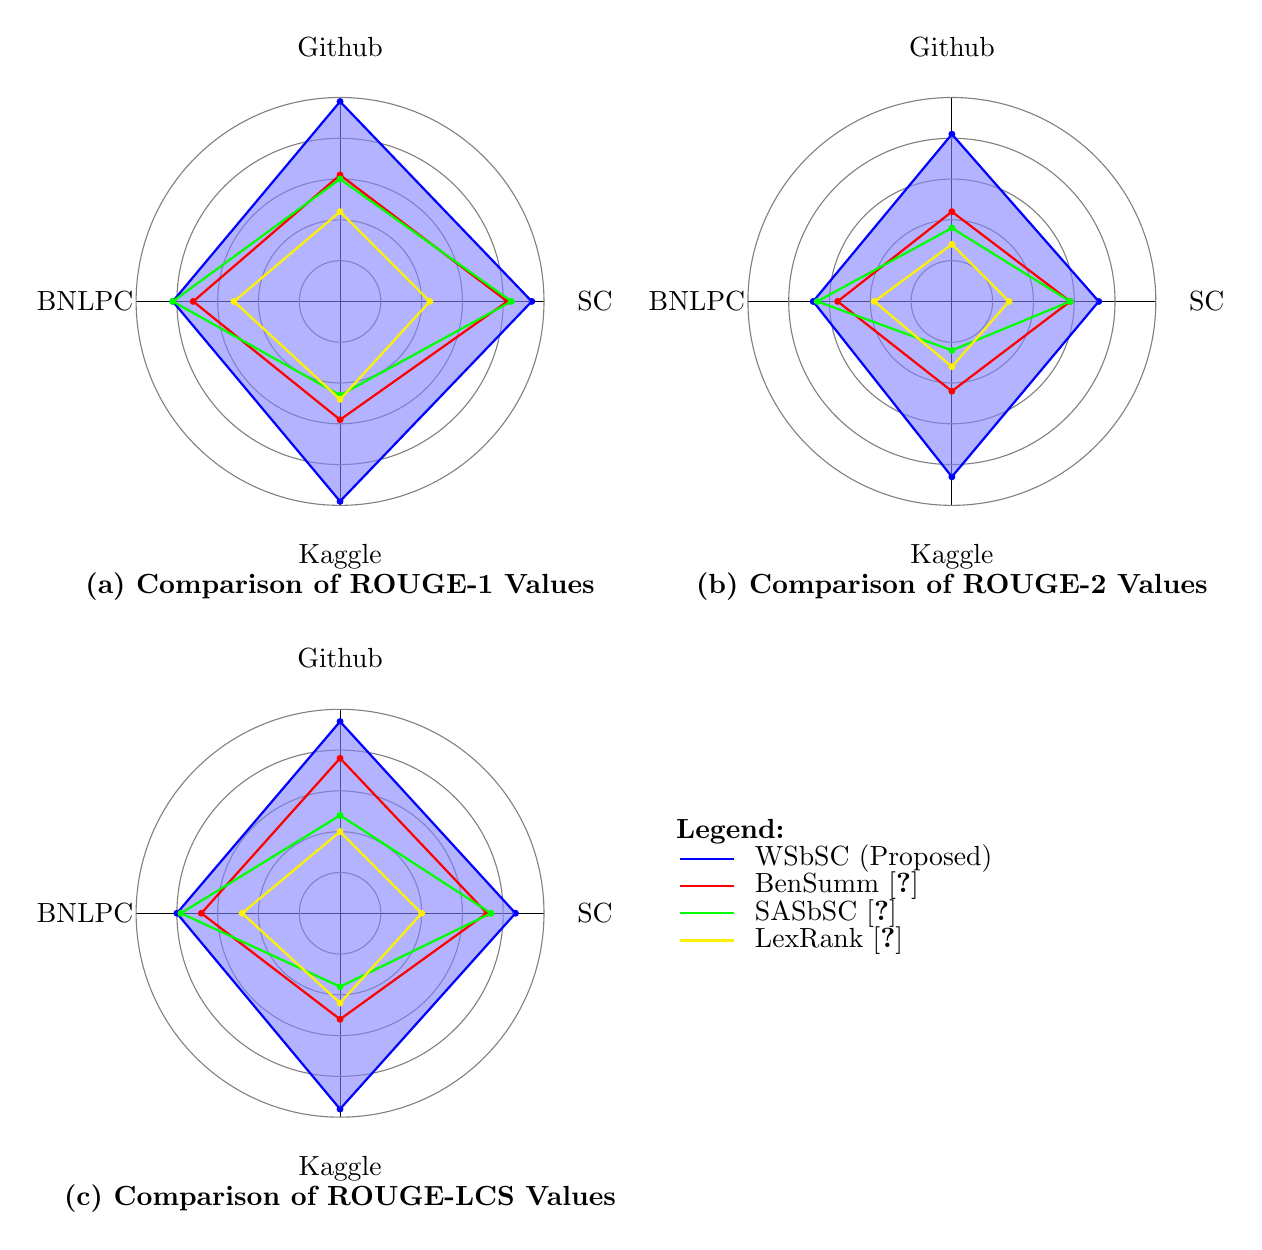
\begin{tikzpicture}[scale=0.0025*\textwidth]
    % Define the number of axes (dimensions)
    \def\n{4}
    % Define the names of the features
    \def\features{{"SC", "Kaggle", "BNLPC", "Github"}}
    % Define the maximum value
    \def\maxvalue{5}

    % Define values for three different radar charts
    \def\valuesAW{{4.7, 4.9, 4.1, 4.9}}
    \def\valuesAB{{4.1, 2.9, 3.6, 3.1}}
    \def\valuesAS{{4.2, 2.3, 4.1, 3.0}}
    \def\valuesAL{{2.2, 2.4, 2.6, 2.2}}

    \def\valuesBW{{3.6, 4.3, 3.4, 4.1}}
    \def\valuesBB{{2.9, 2.2, 2.8, 2.2}}
    \def\valuesBS{{2.9, 1.2, 3.3, 1.8}}
    \def\valuesBL{{1.4, 1.6, 1.9, 1.4}}

    \def\valuesCW{{4.3, 4.8, 4.0, 4.7}}
    \def\valuesCB{{3.6, 2.6, 3.4, 3.8}}
    \def\valuesCS{{3.7, 1.8, 3.9, 2.4}}
    \def\valuesCL{{2.0, 2.2, 2.4, 2.0}}

    % First Radar Chart (Top-left quarter)
    \begin{scope}[xshift=-5cm, yshift=5cm, scale=0.6]
        %write the dataset labels
        \foreach \i in {1,...,\n} {
            \draw (90-\i*360/\n:5) -- (0,0);
            \node at (90-\i*360/\n:6.25) {\pgfmathparse{\features[\i-1]}\pgfmathresult};
        }
        %draw the circle
        \node at (90-2*360/4:7){\textbf{(a) Comparison of ROUGE-1 Values}};
        \foreach \j in {1,...,\maxvalue} {
            \draw[gray, thin] (0,0) circle (\j);
        }

        %draw wsbsc
        \foreach \i [evaluate={\angle=90-\i*360/\n; \valueAW=\valuesAW[\i-1];}] in {1,...,\n} {
            \coordinate (PA\i) at (\angle:\valueAW);
            \filldraw[blue] (PA\i) circle (2pt);
        }
        \fill[blue!50, opacity=0.6] (PA1) -- (PA2) -- (PA3) -- (PA4) -- cycle;
        \foreach \i in {1,...,\n} {
            \pgfmathtruncatemacro{\nexti}{mod(\i,\n)+1}
%                    \draw [thick, cyan] plot [smooth, tension=2] coordinates { (PA\i) (PA\nexti)};
            \draw[thick, blue] (PA\i) -- (PA\nexti);
        }
%                \draw [thick,cyan] plot [smooth cycle, tension=1] coordinates { (PA1) (PA2) (PA3) (PA4)};

        %draw bensumm
        \foreach \i [evaluate={\angle=90-\i*360/\n; \valueAB=\valuesAB[\i-1];}] in {1,...,\n} {
            \coordinate (PB\i) at (\angle:\valueAB);
            \filldraw[red] (PB\i) circle (2pt);
        }
        \foreach \i in {1,...,\n} {
            \pgfmathtruncatemacro{\nexti}{mod(\i,\n)+1}
            \draw[thick, red] (PB\i) -- (PB\nexti);
        }

%                draw sasbsc
        \foreach \i [evaluate={\angle=90-\i*360/\n; \valueAS=\valuesAS[\i-1];}] in {1,...,\n} {
            \coordinate (PC\i) at (\angle:\valueAS);
            \filldraw[green] (PC\i) circle (2pt);
        }
        \foreach \i in {1,...,\n} {
            \pgfmathtruncatemacro{\nexti}{mod(\i,\n)+1}
            \draw[thick, green] (PC\i) -- (PC\nexti);
        }

        %draw lexrank
        \foreach \i [evaluate={\angle=90-\i*360/\n; \valueAL=\valuesAL[\i-1];}] in {1,...,\n} {
            \coordinate (PD\i) at (\angle:\valueAL);
            \filldraw[yellow] (PD\i) circle (2pt);
        }
        \foreach \i in {1,...,\n} {
            \pgfmathtruncatemacro{\nexti}{mod(\i,\n)+1}
            \draw[thick, yellow] (PD\i) -- (PD\nexti);
        }
    \end{scope}

    % Second Radar Chart (Top-right quarter)
    \begin{scope}[xshift=4cm, yshift=5cm, scale=0.6]
        \foreach \i in {1,...,\n} {
            \draw (90-\i*360/\n:5) -- (0,0);
            \node at (90-\i*360/\n:6.25) {\pgfmathparse{\features[\i-1]}\pgfmathresult};
        }
        \node at (90-2*360/4:7){\textbf{(b) Comparison of ROUGE-2 Values}};
        \foreach \j in {1,...,\maxvalue} {
            \draw[gray, thin] (0,0) circle (\j);
        }

        \foreach \i [evaluate={\angle=90-\i*360/\n; \valueBW=\valuesBW[\i-1];}] in {1,...,\n} {
            \coordinate (PA\i) at (\angle:\valueBW);
            \filldraw[blue] (PA\i) circle (2pt);
        }
        \fill[blue!50, opacity=0.6] (PA1) -- (PA2) -- (PA3) -- (PA4) -- cycle;
        \foreach \i in {1,...,\n} {
            \pgfmathtruncatemacro{\nexti}{mod(\i,\n)+1}
            \draw[thick, blue] (PA\i) -- (PA\nexti);
        }

        \foreach \i [evaluate={\angle=90-\i*360/\n; \valueBB=\valuesBB[\i-1];}] in {1,...,\n} {
            \coordinate (PB\i) at (\angle:\valueBB);
            \filldraw[red] (PB\i) circle (2pt);
        }
        \foreach \i in {1,...,\n} {
            \pgfmathtruncatemacro{\nexti}{mod(\i,\n)+1}
            \draw[thick, red] (PB\i) -- (PB\nexti);
        }

        \foreach \i [evaluate={\angle=90-\i*360/\n; \valueBS=\valuesBS[\i-1];}] in {1,...,\n} {
            \coordinate (PC\i) at (\angle:\valueBS);
            \filldraw[green] (PC\i) circle (2pt);
        }
        \foreach \i in {1,...,\n} {
            \pgfmathtruncatemacro{\nexti}{mod(\i,\n)+1}
            \draw[thick, green] (PC\i) -- (PC\nexti);
        }

        \foreach \i [evaluate={\angle=90-\i*360/\n; \valueBL=\valuesBL[\i-1];}] in {1,...,\n} {
            \coordinate (PD\i) at (\angle:\valueBL);
            \filldraw[yellow] (PD\i) circle (2pt);
        }
        \foreach \i in {1,...,\n} {
            \pgfmathtruncatemacro{\nexti}{mod(\i,\n)+1}
            \draw[thick, yellow] (PD\i) -- (PD\nexti);
        }
    \end{scope}

    % Third Radar Chart (Bottom-left quarter)
    \begin{scope}[xshift=-5cm, yshift=-4cm, scale=0.6]
        \foreach \i in {1,...,\n} {
            \draw (90-\i*360/\n:5) -- (0,0);
            \node at (90-\i*360/\n:6.25) {\pgfmathparse{\features[\i-1]}\pgfmathresult};
        }
        \node at (90-2*360/4:7){\textbf{(c) Comparison of ROUGE-LCS Values}};
        \foreach \j in {1,...,\maxvalue} {
            \draw[gray, thin] (0,0) circle (\j);
        }

        \foreach \i [evaluate={\angle=90-\i*360/\n; \valueCW=\valuesCW[\i-1];}] in {1,...,\n} {
            \coordinate (PA\i) at (\angle:\valueCW);
            \filldraw[blue] (PA\i) circle (2pt);
        }
        \fill[blue!50, opacity=0.6] (PA1) -- (PA2) -- (PA3) -- (PA4) -- cycle;
        \foreach \i in {1,...,\n} {
            \pgfmathtruncatemacro{\nexti}{mod(\i,\n)+1}
            \draw[thick, blue] (PA\i) -- (PA\nexti);
        }

        \foreach \i [evaluate={\angle=90-\i*360/\n; \valueCB=\valuesCB[\i-1];}] in {1,...,\n} {
            \coordinate (PB\i) at (\angle:\valueCB);
            \filldraw[red] (PB\i) circle (2pt);
        }
        \foreach \i in {1,...,\n} {
            \pgfmathtruncatemacro{\nexti}{mod(\i,\n)+1}
            \draw[thick, red] (PB\i) -- (PB\nexti);
        }

        \foreach \i [evaluate={\angle=90-\i*360/\n; \valueCS=\valuesCS[\i-1];}] in {1,...,\n} {
            \coordinate (PC\i) at (\angle:\valueCS);
            \filldraw[green] (PC\i) circle (2pt);
        }
        \foreach \i in {1,...,\n} {
            \pgfmathtruncatemacro{\nexti}{mod(\i,\n)+1}
            \draw[thick, green] (PC\i) -- (PC\nexti);
        }

        \foreach \i [evaluate={\angle=90-\i*360/\n; \valueCL=\valuesCL[\i-1];}] in {1,...,\n} {
            \coordinate (PD\i) at (\angle:\valueCL);
            \filldraw[yellow] (PD\i) circle (2pt);
        }
        \foreach \i in {1,...,\n} {
            \pgfmathtruncatemacro{\nexti}{mod(\i,\n)+1}
            \draw[thick, yellow] (PD\i) -- (PD\nexti);
        }
    \end{scope}

    % Legend (Bottom-right quarter)
    \begin{scope}[xshift=4cm, yshift=-4cm, scale=0.8]
        \node[anchor=west] at (-5.25, 1.5) {\textbf{Legend:}};
        \draw[thick, blue] (-5, 1) -- (-4, 1);
        \node[anchor=west] at (-3.8, 1) {WSbSC (Proposed)};

        \draw[thick, red] (-5, 0.5) -- (-4, 0.5);
        \node[anchor=west] at (-3.8, 0.5) {BenSumm~\cite{chowdhury-etal-2021-tfidf-clustering}};

        \draw[thick, green] (-5, 0) -- (-4, 0);
        \node[anchor=west] at (-3.8, 0) {SASbSC~\cite{roychowdhury-etal-2022-spectral-base}};

        \draw[thick, yellow] (-5, -0.5) -- (-4, -0.5);
        \node[anchor=west] at (-3.8, -0.5) {LexRank~\cite{Erkan-lexRank-2004}};
    \end{scope}
\end{tikzpicture}
    \caption{The Radar chart of the models of being compared on four datasets at once}
    \label{fig:radarchart}
\end{figure}
\begin{figure}
    \centering
    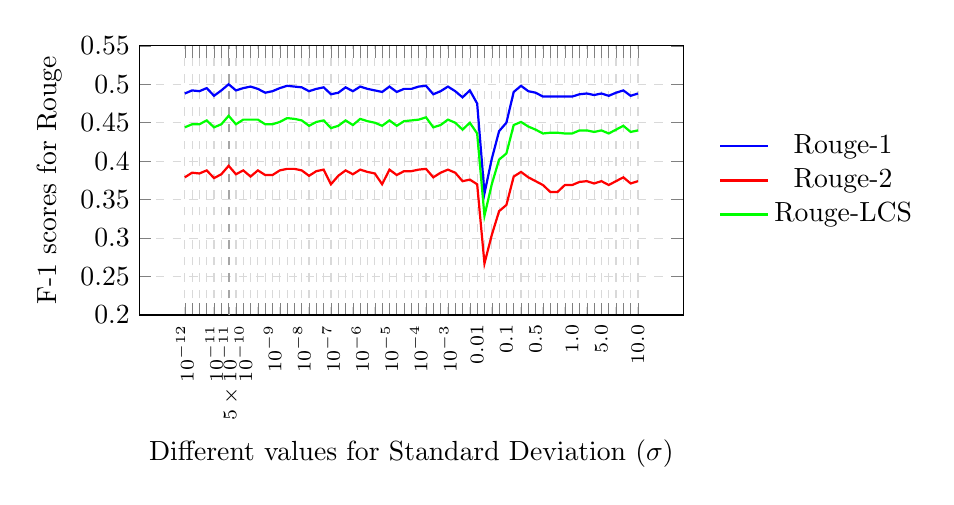
\begin{tikzpicture}
    \begin{axis}[
        width=.7\textwidth,
        height=5cm,
        xlabel={Different values for Standard Deviation ($\sigma$)},
        ylabel={F-1 scores for Rouge},
        ymin=0.2, ymax=0.55,
        xtick={1,2,...,63}, % Original 63 ticks
        xticklabels={ $10^{-12}$, , , , $10^{-11}$, ,$5\times10^{-11}$, , $10^{-10}$, , , , $10^{-9}$, , , , $10^{-8}$, , , ,
                     $10^{-7}$, , , , $10^{-6}$, , , , $10^{-5}$, , , , $10^{-4}$, , , ,
                     $10^{-3}$, , , , $0.01$, , , , $0.1$, , , , $0.5$, , , ,
                      , $1.0$, , , , $5.0$, , , , ,$10.0$}, % Show 1 in every 4 labels
        xticklabel style={rotate=90, anchor=east, font=\scriptsize}, % Rotate labels 90 degrees
        legend style={at={(1.05,0.5)}, anchor=west, draw=none}, % Move legend outside, remove border
        extra x ticks={7}, % Add extra tick for 7th position
        extra x tick style={grid=major, major grid style={gray!70, thick}}, % Style for the highlighted tic
        extra x tick labels={},
        grid=major,
        grid style={dashed,gray!30},
        ytick={0.20, 0.25, 0.30, 0.35, 0.40, 0.45, 0.50, 0.55}, % Y-axis ticks
        cycle list name=color list,
    ]

    % Dummy data for Column 1
    \addplot[color=blue, thick] coordinates {
        (1, 0.488)
        (2, 0.492)
        (3, 0.491)
        (4, 0.495)
        (5, 0.485)
        (6, 0.492)
        (7, 0.500)
        (8, 0.492)
        (9, 0.495)
        (10, 0.497)
        (11, 0.494)
        (12, 0.489)
        (13, 0.491)
        (14, 0.495)
        (15, 0.498)
        (16, 0.497)
        (17, 0.496)
        (18, 0.491)
        (19, 0.494)
        (20, 0.496)
        (21, 0.487)
        (22, 0.489)
        (23, 0.496)
        (24, 0.491)
        (25, 0.497)
        (26, 0.494)
        (27, 0.492)
        (28, 0.490)
        (29, 0.497)
        (30, 0.490)
        (31, 0.494)
        (32, 0.494)
        (33, 0.497)
        (34, 0.498)
        (35, 0.487)
        (36, 0.491)
        (37, 0.497)
        (38, 0.491)
        (39, 0.483)
        (40, 0.492)
        (41, 0.475)
        (42, 0.358)
        (43, 0.403)
        (44, 0.439)
        (45, 0.450)
        (46, 0.490)
        (47, 0.498)
        (48, 0.491)
        (49, 0.489)
        (50, 0.484)
        (51, 0.484)
        (52, 0.484)
        (53, 0.484)
        (54, 0.484)
        (55, 0.487)
        (56, 0.488)
        (57, 0.486)
        (58, 0.488)
        (59, 0.485)
        (60, 0.489)
        (61, 0.492)
        (62, 0.485)
        (63, 0.488)
    };
    \addlegendentry{Rouge-1}

    % Dummy data for Column 2
    \addplot[color=red, thick] coordinates {
        (1, 0.379)
        (2, 0.385)
        (3, 0.384)
        (4, 0.388)
        (5, 0.378)
        (6, 0.383)
        (7, 0.394)
        (8, 0.383)
        (9, 0.388)
        (10, 0.380)
        (11, 0.388)
        (12, 0.382)
        (13, 0.382)
        (14, 0.388)
        (15, 0.390)
        (16, 0.390)
        (17, 0.388)
        (18, 0.381)
        (19, 0.387)
        (20, 0.389)
        (21, 0.370)
        (22, 0.381)
        (23, 0.388)
        (24, 0.383)
        (25, 0.389)
        (26, 0.386)
        (27, 0.384)
        (28, 0.370)
        (29, 0.389)
        (30, 0.382)
        (31, 0.387)
        (32, 0.387)
        (33, 0.389)
        (34, 0.390)
        (35, 0.379)
        (36, 0.385)
        (37, 0.389)
        (38, 0.385)
        (39, 0.374)
        (40, 0.376)
        (41, 0.370)
        (42, 0.267)
        (43, 0.304)
        (44, 0.335)
        (45, 0.343)
        (46, 0.380)
        (47, 0.386)
        (48, 0.379)
        (49, 0.374)
        (50, 0.369)
        (51, 0.360)
        (52, 0.360)
        (53, 0.369)
        (54, 0.369)
        (55, 0.373)
        (56, 0.374)
        (57, 0.371)
        (58, 0.374)
        (59, 0.369)
        (60, 0.374)
        (61, 0.379)
        (62, 0.371)
        (63, 0.374)
    };
    \addlegendentry{Rouge-2}

    % Dummy data for Column 3
    \addplot[color=green, thick] coordinates {
        (1, 0.444)
        (2, 0.448)
        (3, 0.448)
        (4, 0.453)
        (5, 0.444)
        (6, 0.448)
        (7, 0.459)
        (8, 0.448)
        (9, 0.454)
        (10, 0.454)
        (11, 0.454)
        (12, 0.448)
        (13, 0.448)
        (14, 0.451)
        (15, 0.456)
        (16, 0.455)
        (17, 0.453)
        (18, 0.446)
        (19, 0.451)
        (20, 0.453)
        (21, 0.443)
        (22, 0.446)
        (23, 0.453)
        (24, 0.447)
        (25, 0.455)
        (26, 0.452)
        (27, 0.450)
        (28, 0.446)
        (29, 0.453)
        (30, 0.446)
        (31, 0.452)
        (32, 0.453)
        (33, 0.454)
        (34, 0.457)
        (35, 0.444)
        (36, 0.447)
        (37, 0.454)
        (38, 0.450)
        (39, 0.441)
        (40, 0.450)
        (41, 0.436)
        (42, 0.329)
        (43, 0.370)
        (44, 0.402)
        (45, 0.410)
        (46, 0.447)
        (47, 0.451)
        (48, 0.445)
        (49, 0.441)
        (50, 0.436)
        (51, 0.437)
        (52, 0.437)
        (53, 0.436)
        (54, 0.436)
        (55, 0.440)
        (56, 0.440)
        (57, 0.438)
        (58, 0.440)
        (59, 0.436)
        (60, 0.441)
        (61, 0.446)
        (62, 0.438)
        (63, 0.440)
    };
    \addlegendentry{Rouge-LCS}

    \end{axis}
\end{tikzpicture}
    \caption{Fine-tuning for different standard deviation~($\sigma$)~values}
    \label{fig:sigma-fine-tuning}
\end{figure}

\subsubsection{Different Ranking Techniques Inside Clusters}\label{subsubsec:different-ranking-techniques-inside-clusters}
We implemented two ranking methods to pick the best sentence from each cluster. The first one is the First Rank method where we just pick the sentence that appears first in the input document. The second one is the TF-IDF ranking, where we ranked the sentences by their TF-IDF scores and pick the best one. We can see in the table~\ref{tab:ranking} that the TF-IDF performs better on a high quality dataset like our Self-curated one.

\begin{table}[]
    \centering
    \begin{tabular}{cccc}\hline
        Method      & Rouge-1       & Rouge-2       & Rouge-LCS     \\\hline
        FirstRank   & 0.47          & 0.36          & 0.43          \\
        TF-IDF      & \textbf{0.50} & \textbf{0.40} & \textbf{0.46} \\\hline
    \end{tabular}
    \caption{Comparison of Result of different ranking techniques}
    \label{tab:ranking}
\end{table}

\subsection{Implementation Into Other Languages}\label{subsec:implementation-into-other-languages}
The proposed model is not language-dependent, thus it can be extended into other languages. To perform this method into a language, we only need a language-specific tokenizer, a list of stop-words and a word vector embedding dataset. We tried to find quality extractive text summarization dataset for evaluating the method, but could only find relevant datasets in three other languages i.e., Hindi, Marathi and Turkish. We adopted this Model into these three low resource languages to check this hypothesis.\\

\begin{table}[]
    \centering
    \begin{tabular}{cccc}\hline
        Language                & Rouge-1   & Rouge-2   & Rouge-LCS \\\hline
        Bengali (Dataset - 1)   & 0.47      & 0.36      & 0.43      \\
        Bengali (Dataset - 2)   & 0.49      & 0.43      & 0.48      \\
        Bengali (Dataset - 3)   & 0.41      & 0.34      & 0.40      \\
        Bengali (Dataset - 4)   & 0.49      & 0.41      & 0.47      \\
        Bengali (Average)       & 0.47      & 0.38      & 0.44      \\\hline
        Hindi                   & 0.40      & 0.26      & 0.36      \\\hline
        Marathi                 & 0.50	    & 0.42      & 0.50      \\\hline
        Turkish                 & 0.48      & 0.39      & 0.47      \\\hline
    \end{tabular}
    \caption{Comparison of Result of proposed summarization method in other low-resource languages}
    \label{tab:other_language}
\end{table}

The Table-\ref{tab:other_language} shows the result of the proposed word similarity based spectral clustering method for extractive summarization in other low resource languages. For the Hindi language, we used a Kaggle dataset\footnote{\textit{https://www.kaggle.com/datasets/disisbig/hindi-text-short-and-large-summarization-corpus/}} produced by Gaurav Arora. For the Marathi language, we used another Kaggle dataset\footnote{\textit{https://www.kaggle.com/datasets/ketki19/marathi}} produced by Ketki Nirantar. For the Turkish language, we used a GitHub dataset\footnote{\textit{https://github.com/xtinge/turkish-extractive-summarization-dataset/blob/main/dataset/XTINGE-SUM\_TR\_EXT/xtinge-sum\_tr\_ext.json}} produced by the XTINGE~\cite{Demir-2024-xtinge_turkish_extractive} team. We can see that the results on Marathi and Turkish are slightly better than the result on Bengali. Although it performs slightly lower on Hindi, The score is still similar to Bengali.
